\section{Публичный api}
В данном разделе описаны классы и интерфейсы, которые предоставляют внешний пользовательский механизм по работе с библиотекой JMantic

% \subsection{Интерфейсы типов}

\subsection{DefaultScContext}
Данный тип Sc-контекста является рекомендуемым к использованию, так как данная реализация поддерживает наиболее актуальные методы и полностью реализует типобезопасность java. Кроме этого, вынуждает пользователя обрабатывать исключения, выбрасываемые ScMemory. 


DefaultScContext предоставляет программисту следующие методы:

\subsubsection{createNode} 

Создание узла заданного типа. Данный метод создаёт узел в sc-памяти и возвращает объект, который является реализацией интерфейса ScNode. Полученный объект имеет адрес и тип.
\subsubsection {createNodes} 

Создание группы узлов. Данный метод позволяет оптимизировать групповые запросы создания узлов. При создании узла по одному, происходит генерация json-а, отправка на сервер остис, разбор ответа для каждого узла лично. В групповом же варианте создаётся только один json-запрос. 
\subsubsection {createEdge} 

Создание дуги заданного типа между заданным sc-элементами. Данный метод создаёт в sc-памяти sc-дугу и возвращает объект, который является реализацией интерфейса ScEdge. Полученный объект имеет адрес, тип, а также адреса двух sc-элементов, между которыми находится данная дуга.
\subsubsection {createEdges} 

Создание группы дуг. Данный метод позволяет оптимизировать групповые запросы создания дуг. При создании узла по одному, происходит генерация json-а, отправка на сервер остис, разбор ответа для каждой дуги лично. В групповом же варианте создаётся только один json-запрос. 
\subsubsection {createIntegerLink} 

Создание sc-link для хранения целочисленных значений. Данный метод создаёт в sc-памяти объект типа ScLink с целочисленным содержимым и устанавливает некоторое значение. Возвращает же метод одну из реализаций интерфейса {ScIntegerLink}, которая имеет адрес, тип хранимого значения и само хранимое значение. 
\subsubsection {createFloatLink} 

Создание sc-link для хранения дробных значений. Данный метод создаёт в sc-памяти объект типа ScLink с дробным содержимым и устанавливает некоторое значение. Возвращает же метод одну из реализаций интерфейса ScFloatLink, которая имеет адрес, тип хранимого значения и само хранимое значение. 
\subsubsection {createStringLink} 

Создание sc-link для хранения целочисленных значений. Данный метод создаёт в sc-памяти объект типа ScLink с целочисленным содержимым и устанавливает некоторое значение. Возвращает же метод одну из реализаций интерфейса ScIntegerLink, которая имеет адрес, тип хранимого значения и само хранимое значение. 
\subsubsection {deleteElement} 

Удаление любого ScElement. Данный метод удаляет sc-элемент из sc-памяти по адресу элемента. Возвращает метод логическое значение: true, если удаление прошло успешно; false, если закончилось с ошибкой. 
\subsubsection {deleteElements} 

Удаление группы элементов. Данный метод позволяет оптимизировать групповые запросы удаления элементов. При удалении элементов по одному, происходит генерация json-а, отправка на сервер остис, разбор ответа для каждого элемента лично. В групповом же варианте создаётся только один json-запрос. 
\subsubsection {findAllConstructionsNodeEdgeNode}

Поиск всех конструкций вида узел-дуга-узел. Данный метод принимает один константный узел, относительно которого будет производиться поиск, а также тип искомой дуги и тип искомого узла. Метод вернёт список найденных конструкций, а если точнее, метод вернёт список из объектов-реализаций интерфейса ScEdge. Из данных объектов можно получить соседние узлы. 
\begin{figure}[H]
    \centering
    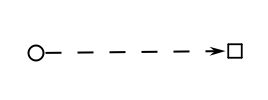
\includegraphics{images/sc-context/node-edge-node.png}
    \caption{Пример искомой конструкции}
    \label{json_ex}
\end{figure}
\subsubsection {findAllConstructionsNodeEdgeLink} (Удалён. Заменён на универсальные поисковые шаблоны конструкций на 3)

Поиск всех конструкций вида узел-дуга-sclink. Данный метод принимает один константный узел, относительно которого будет производиться поиск, а также тип искомой дуги, тип искомой sclink и тип содержимого искомой sclink. Метод вернёт список найденных конструкций, а если точнее, метод вернёт список из объектов-реализаций интерфейса ScEdge. Из данных объектов можно получить соседние элементы. 
\begin{figure}[H]
    \centering
    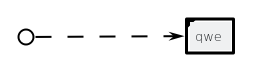
\includegraphics{images/sc-context/node-edge-link.png}
    \caption{Пример искомой конструкции}
    \label{json_ex}
\end{figure}

\subsubsection {findAllConstructionsNodeEdgeLinkWithRelation} (Удалён. Заменён на универсальные поисковые шаблоны конструкций на 5)

Поиск всех конструкций вида узел-дуга-sclink. Данный метод принимает один константный узел, относительно которого будет производиться поиск, а также тип искомой дуги, тип искомой sclink, тип содержимого искомой sclink, адрес узла-отношения, тип дуги отношения. Метод вернёт список найденных конструкций, а если точнее, метод вернёт список из объектов-реализаций интерфейса ScEdge. Из данных объектов можно получить соседние элементы. 
\begin{figure}[H]
    \centering
    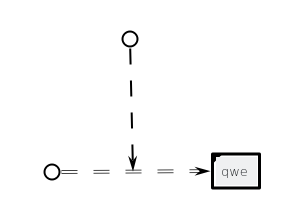
\includegraphics{images/sc-context/node-edge-link-with-rel.png}
    \caption{Пример искомой конструкции}
    \label{json_ex}
\end{figure}

\subsubsection{find(ScPattern3)} 

Поиск всех конструкций по шаблону на 3 элемента. Данный метод принимает один шаблон и возвращает список найденных конструкций (также на 3 элемента). Для создания шаблона можно воспользоваться как обычным использованием класса ScPattern3Impl (то есть, ручным заполнением правил поиска), так и, что более предпочтительно, с помощью фабрик DefaultScPattern3Factory, ScPattern3FactoryWithNames. 


\subsubsection{find(ScPattern5)} 

Поиск всех конструкций по шаблону на 5 элементов. Данный метод принимает один шаблон и возвращает список найденных конструкций (также на 5 элементов). Для создания шаблона можно воспользоваться как обычным использованием класса ScPattern5Impl (то есть, ручным заполнением правил поиска), так и, что более предпочтительно, с помощью фабрик DefaultScPattern5Factory, ScPattern5FactoryWithNames. 


\subsubsection{find(ScPattern)} 

Поиск всех конструкций по универсальному шаблону. Данный метод принимает один шаблон и возвращает список найденных конструкций (количество элементов в конструкции будет равно количеству найденных по шаблону элементов). Создать шаблон можно только вручную с помощью одной из имплементаций (на данный момент - DefaultWebsocketScPattern).

\subsubsection {setIntegerLinkContent} 

Задание значения sclink. Данный метод задаёт целочисленное значения в ScIntegerLink в sc-памяти. Возвращает метод логическое значение: true, если операция прошла успешно; false, если закончилось с ошибкой. 

\subsubsection {setFloatLinkContent} З

адание значения sclink. Данный метод задаёт дробное значения в ScFloatLink в sc-памяти. Возвращает метод логическое значение: true, если операция прошла успешно; false, если закончилось с ошибкой. 

\subsubsection {setStringLinkContent} 

Задание значения sclink. Данный метод задаёт строковое значения в ScStringLink в sc-памяти. Возвращает метод логическое значение: true, если операция прошла успешно; false, если закончилось с ошибкой. 

\subsubsection {getIntegerLinkContent} 

Получение значения sclink. Данный метод служит для получения актуального целочисленного значения данной ScIntegerLink, делая запрос в базу. Однако, значение, хранимое в sclink можно также получить вызовом метода getContent. В этом случае не гарантируется то, что значение в sclink совпадает со значением в sc-памяти.

\subsubsection {getFloatLinkContent} 

Получение значения sclink. Данный метод служит для получения актуального дробного значения данной ScFloatrLink, делая запрос в базу. Однако, значение, хранимое в sclink можно также получить вызовом метода getContent. В этом случае не гарантируется то, что значение в sclink совпадает со значением в sc-памяти.

\subsubsection {getStringLinkContent} 

Получение значения sclink. Данный метод служит для получения актуального целочисленного значения данной ScStringLink, делая запрос в базу. Однако, значение, хранимое в sclink можно также получить вызовом метода getContent. В этом случае не гарантируется то, что значение в sclink совпадает со значением в sc-памяти.

\subsubsection{findKeynode}

Поиск ключевых узлов. Данный метод служит для нахождения ключевого узла по заданному идентификатору. Принимает в параметрах строку -- идентификатор, а возвращает Optional, который либо содержит в себе найденный узел, либо пуст, если переданный идентификатор не существует в базе. 

\subsubsection{resolveKeynode}

Поиск и создание ключевых узлов. Данный метод служит для нахождения ключевого узла по заданному идентификатору. Принимает в параметрах строку и тип узла -- идентификатор и тип создаваемого узла соответственно. Если узел с данным идентификатором существует, метод вернёт этот узел. В случае, если не существует, будет создан новый узел с заданными идентификатором и типом узла. 

\subsection{UncheckedScContext}
Данный тип Sc-контекста не рекомендуется к реальному использованию, так как скрывает исключения, выбрасываемые в ScMemory. Этот Sc-контекст удобно использовать для демонстрации работы и тестирования, ведь позволяет не оборачивать все методы в блоки try-catch. 

В данном контексте приведены следующие методы:
\subsubsection{createNode} 
Создание узла заданного типа. Данный метод создаёт узел в sc-памяти и возвращает объект, который является реализацией интерфейса ScNode. Полученный объект имеет адрес и тип.

\subsubsection {createNodes} Создание группы узлов. Данный метод позволяет оптимизировать групповые запросы создания узлов. При создании узла по одному, происходит генерация json-а, отправка на сервер остис, разбор ответа для каждого узла лично. В групповом же варианте создаётся только один json-запрос. 
\subsubsection {createEdge} Создание дуги заданного типа между заданным sc-элементами. Данный метод создаёт в sc-памяти sc-дугу и возвращает объект, который является реализацией интерфейса ScEdge. Полученный объект имеет адрес, тип, а также адреса двух sc-элементов, между которыми находится данная дуга.
\subsubsection {createEdges} Создание группы дуг. Данный метод позволяет оптимизировать групповые запросы создания дуг. При создании узла по одному, происходит генерация json-а, отправка на сервер остис, разбор ответа для каждой дуги лично. В групповом же варианте создаётся только один json-запрос. 
\subsubsection {createIntegerLink} Создание sc-link для хранения целочисленных значений. Данный метод создаёт в sc-памяти объект типа ScLink с целочисленным содержимым и устанавливает некоторое значение. Возвращает же метод одну из реализаций интерфейса {ScIntegerLink}, которая имеет адрес, тип хранимого значения и само хранимое значение. 
\subsubsection {createFloatLink} Создание sc-link для хранения дробных значений. Данный метод создаёт в sc-памяти объект типа ScLink с дробным содержимым и устанавливает некоторое значение. Возвращает же метод одну из реализаций интерфейса ScFloatLink, которая имеет адрес, тип хранимого значения и само хранимое значение. 
\subsubsection {createStringLink} Создание sc-link для хранения целочисленных значений. Данный метод создаёт в sc-памяти объект типа ScLink с целочисленным содержимым и устанавливает некоторое значение. Возвращает же метод одну из реализаций интерфейса ScIntegerLink, которая имеет адрес, тип хранимого значения и само хранимое значение. 
\subsubsection {deleteElement} Удаление любого ScElement. Данный метод удаляет sc-элемент из sc-памяти по адресу элемента. Возвращает метод логическое значение: true, если удаление прошло успешно; false, если закончилось с ошибкой. 
\subsubsection {deleteElements} Удаление группы элементов. Данный метод позволяет оптимизировать групповые запросы удаления элементов. При удалении элементов по одному, происходит генерация json-а, отправка на сервер остис, разбор ответа для каждого элемента лично. В групповом же варианте создаётся только один json-запрос. 
\subsubsection {findAllConstructionsNodeEdgeNode} Поиск всех конструкций вида узел-дуга-узел. Данный метод принимает один константный узел, относительно которого будет производиться поиск, а также тип искомой дуги и тип искомого узла. Метод вернёт список найденных конструкций, а если точнее, метод вернёт список из объектов-реализаций интерфейса ScEdge. Из данных объектов можно получить соседние узлы. 
\begin{figure}[H]
    \centering
    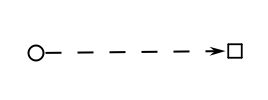
\includegraphics{images/sc-context/node-edge-node.png}
    \caption{Пример искомой конструкции}
    \label{json_ex}
\end{figure}

\subsubsection{find(ScPattern3)} 

Поиск всех конструкций по шаблону на 3 элемента. Данный метод принимает один шаблон и возвращает список найденных конструкций (также на 3 элемента). Для создания шаблона можно воспользоваться как обычным использованием класса ScPattern3Impl (то есть, ручным заполнением правил поиска), так и, что более предпочтительно, с помощью фабрик DefaultScPattern3Factory, ScPattern3FactoryWithNames. 


\subsubsection{find(ScPattern5)} 

Поиск всех конструкций по шаблону на 5 элементов. Данный метод принимает один шаблон и возвращает список найденных конструкций (также на 5 элементов). Для создания шаблона можно воспользоваться как обычным использованием класса ScPattern5Impl (то есть, ручным заполнением правил поиска), так и, что более предпочтительно, с помощью фабрик DefaultScPattern5Factory, ScPattern5FactoryWithNames. 


\subsubsection{find(ScPattern)} 

Поиск всех конструкций по универсальному шаблону. Данный метод принимает один шаблон и возвращает список найденных конструкций (количество элементов в конструкции будет равно количеству найденных по шаблону элементов). Создать шаблон можно только вручную с помощью одной из имплементаций (на данный момент - DefaultWebsocketScPattern).


\subsubsection {setIntegerLinkContent} Задание значения sclink. Данный метод задаёт целочисленное значения в ScIntegerLink в sc-памяти. Возвращает метод логическое значение: true, если операция прошла успешно; false, если закончилось с ошибкой. 
\subsubsection {setFloatLinkContent} Задание значения sclink. Данный метод задаёт дробное значения в ScFloatLink в sc-памяти. Возвращает метод логическое значение: true, если операция прошла успешно; false, если закончилось с ошибкой. 
\subsubsection {setStringLinkContent} Задание значения sclink. Данный метод задаёт строковое значения в ScStringLink в sc-памяти. Возвращает метод логическое значение: true, если операция прошла успешно; false, если закончилось с ошибкой. 
\subsubsection {getIntegerLinkContent} Получение значения sclink. Данный метод служит для получения актуального целочисленного значения данной ScIntegerLink, делая запрос в базу. Однако, значение, хранимое в sclink можно также получить вызовом метода getContent. В этом случае не гарантируется то, что значение в sclink совпадает со значением в sc-памяти.
\subsubsection {getFloatLinkContent} Получение значения sclink. Данный метод служит для получения актуального дробного значения данной ScFloatrLink, делая запрос в базу. Однако, значение, хранимое в sclink можно также получить вызовом метода getContent. В этом случае не гарантируется то, что значение в sclink совпадает со значением в sc-памяти.
\subsubsection {getStringLinkContent} Получение значения sclink. Данный метод служит для получения актуального целочисленного значения данной ScStringLink, делая запрос в базу. Однако, значение, хранимое в sclink можно также получить вызовом метода getContent. В этом случае не гарантируется то, что значение в sclink совпадает со значением в sc-памяти.

\subsubsection{findKeynode}

Поиск ключевых узлов. Данный метод служит для нахождения ключевого узла по заданному идентификатору. Принимает в параметрах строку -- идентификатор, а возвращает Optional, который либо содержит в себе найденный узел, либо пуст, если переданный идентификатор не существует в базе. 

\subsubsection{resolveKeynode}

Поиск и создание ключевых узлов. Данный метод служит для нахождения ключевого узла по заданному идентификатору. Принимает в параметрах строку и тип узла -- идентификатор и тип создаваемого узла соответственно. Если узел с данным идентификатором существует, метод вернёт этот узел. В случае, если не существует, будет создан новый узел с заданными идентификатором и типом узла. 


\subsection{AsyncUncheckedScContext}
Данный тип Sc-контекста является, в больше степени, эксперементальным. Он, как и контекст UncheckedScContext, скрывает исключения ScMemory, позволяя писать код без блоков try-catch. Также при вызове методов, будет возвращён не результат выполнения метода, а объект Future. То есть, сами вызовы методов не являются блокирующими, что может быть очень полезно в некоторых ситуациях, ведь код java-программы продолжает исполнение не дожидаясь ответа, который занимает сотни миллисекунд. 

Все доступные методы и их описания совпадают с методы в UncheckedScContext. 